% !TeX root = ../../Book1.tex
% 纲要标题：### 15.2 沿路径的平行移动
% 纲要位置：几何学计划纲要.md，第 701 行。
% 正文状态：初稿；尚未正式审核。

% 纲要内容开始
% 
% * 协变常微分方程及参数依赖
% * 路径拼接、反向和平行移动
% * 由平行移动恢复联络
% * 度量联络和长度保持
% 
% 纲要内容结束

\section{沿路径的平行移动}
\label{g1:sec:1502}

联络规定了截面怎样沿一个瞬时方向变化，但两个不同点处的向量仍属于不同纤维，不能直接相减。如果沿一条路径要求协变导数始终为零，就可以由初始向量确定沿途的“不变”向量。这将给出两个端点纤维之间的线性同构。比较一般截面时，可以先把终点向量运回起点再作差；这个差商又会恢复最初的联络。

\ProseParagraphBreak

本节的底流形 \(M\) 为有限维、Hausdorff、第二可数的光滑流形，允许有边界；\(E\to M\) 是实秩 \(r\) 光滑向量丛，已给定\cref{g1:def:bundle-connection}中的联络 \(\nabla\)。局部标架写成行 \(e=(e_1,\ldots,e_r)\)，截面分量写成列，约定 \(\nabla e=eA\)。存在性所需的分析输入是\cref{g1:thm:ode-local-existence-uniqueness,g1:thm:ode-smooth-dependence}：光滑常微分方程有唯一局部解，且在共同存在区间上光滑依赖初值和有限维参数。我们还要补明，当前的线性方程为何能走完整个给定的紧时间区间。

\subsection{协变常微分方程及参数依赖}
\label{g1:subsec:1502:01}

设 \(\gamma:I\to M\) 是光滑曲线。沿 \(\gamma\) 的一个向量 \(s(t)\) 位于 \(E_{\gamma(t)}\)，所以应当把它看成拉回丛 \(\gamma^*E\to I\) 的截面，参见\cref{g1:prop:pullback-bundle}。具体说，\(s:I\to E\) 光滑且 \(\pi\circ s=\gamma\)。即使 \(\gamma(t_1)=\gamma(t_2)\)，也不要求 \(s(t_1)=s(t_2)\)。因此不能要求每个沿曲线的截面都由底流形上的同一个截面限制而来；自交与常值路径已经会使这种要求失败。

\begin{definition}[沿曲线的协变导数]\label{g1:def:along-curve-covariant-derivative}
	设 \(E\to M\) 为实有限秩光滑向量丛，\(\nabla\) 为联络，\(I\subseteq\mathbb R\) 为区间，\(\gamma:I\to M\) 为光滑曲线，\(s\) 为拉回丛 \(\gamma^*E\) 的光滑截面，\(M\) 可带边界。在曲线落于局部标架 \(e\) 的定义域内的参数子区间上，令 \(\nabla e=eA\)，并写 \(s(t)=e(\gamma(t))u(t)\)，定义
	\begin{equation}\label{g1:eq:along-curve-covariant-derivative}
		\mathrm{D}_t s=e(\gamma(t))\left(\frac{\mathrm{d}u}{\mathrm{d}t}+A_{\gamma(t)}(\gamma'(t))u(t)\right).
	\end{equation}
	这称为 \(s\) 沿 \(\gamma\) 的协变导数。满足 \(\mathrm{D}_t s=0\) 的截面称为沿 \(\gamma\) 的\term[pingxingjiemian]{平行截面}[parallel section]。
\end{definition}

先检验这个定义不依赖标架。若 \(\widetilde e=e g\)、\(u=g(\gamma(t))\widetilde u\)，由\eqref{g1:eq:connection-frame-change}，
\[
	\widetilde A=g^{-1}Ag+g^{-1}\mathrm{d}g.
\]
记 \(B(t)=A_{\gamma(t)}(\gamma'(t))\)、\(g(t)=g(\gamma(t))\)，则 \(\widetilde B=g^{-1}Bg+g^{-1}g'\)，从而
\[
	u'+Bu=g'\widetilde u+g\widetilde u'+Bg\widetilde u
	=g(\widetilde u'+\widetilde B\widetilde u).
\]
乘上 \(e(\gamma(t))\) 后，两套标架给出同一个纤维向量。因此局部公式可以粘合。它也直接给出实线性及乘积法则 \(\mathrm{D}_t(fs)=f's+f\mathrm{D}_ts\)。若 \(S\) 是底流形上的局部截面，则链式法则与\eqref{g1:eq:connection-local-form}说明
\[
	\mathrm{D}_t(S\circ\gamma)=(\nabla_{\gamma'(t)}S)_{\gamma(t)}.
\]
这个相容关系适用于确实来自局部截面的情形，但不是沿曲线导数的定义前提。

\ProseParagraphBreak

现在平行条件成为线性初值问题
\begin{equation}\label{g1:eq:parallel-transport-ode}
	\frac{\mathrm{d}u}{\mathrm{d}t}=-B(t)u(t),\qquad
	B(t)=A_{\gamma(t)}(\gamma'(t)),\qquad u(t_0)=u_0.
\end{equation}
负号来自把联络项移到等式右侧。一般情况下，\(B(t_1)\) 与 \(B(t_2)\) 不交换，因而不能未经验证就把解写成 \(\exp(-\int B)\)。存在唯一性本身并不需要这种显式表达。

\begin{lemma}[线性方程的全区间解]\label{g1:lem:linear-transport-ode}
	设 \(a<b\)，\(B:[a,b]\to\operatorname{Mat}_{r\times r}(\mathbb R)\) 光滑，包括端点处的局部光滑延拓。对任意 \(t_0\in[a,b]\) 与 \(u_0\in\mathbb R^r\)，方程 \(u'=-Bu\)、\(u(t_0)=u_0\) 在整个 \([a,b]\) 上有唯一光滑解。若 \(\|B(t)\|\le L\)，则
	\begin{equation}\label{g1:eq:linear-transport-bound}
		|u(t)|\le e^{L|t-t_0|}|u_0|.
	\end{equation}
	解线性依赖 \(u_0\)。记 \(U(t,s)\) 为从时刻 \(s\) 的分量到时刻 \(t\) 的分量的解算子，则 \(U(t,s)\) 可逆，其逆为 \(U(s,t)\)。若 \(B=B(t,\lambda)\) 光滑依赖有限维参数，解在每个参数点附近对 \(t,t_0,u_0,\lambda\) 联合光滑。
\end{lemma}
\begin{proof}
	局部存在唯一性适用于 \(F(t,u)=-B(t)u\)，因为其右端在时间的局部延拓区间与整个 \(\mathbb R^r\) 上光滑。积分方程给出
	\[
		|u(t)|\le |u_0|+L\int_{t_0}^t|u(v)|\,\mathrm{d}v\qquad(t\ge t_0).
	\]
	\cref{g1:lem:gronwall-estimate}给出\eqref{g1:eq:linear-transport-bound}；向过去求解时先把时间反向，得到相同估计。

	为排除有限时间中断，假设解向前只能存在到 \(c\le b\)。上述界使解在 \([t_0,c)\) 上有共同界 \(C\)，故 \(|u'|\le LC\)。于是 \(|u(t)-u(v)|\le LC|t-v|\)，当 \(t\uparrow c\) 时存在有限极限 \(u_c\)。在 \((c,u_c)\) 处重新使用局部初值定理。旧解的积分方程在 \(c\) 处取极限后仍成立，接上新解便得到穿过 \(c\) 的解，与不能延拓矛盾。若 \(c=b\)，同样得到端点处及其局部延拓中的光滑解。向后完全相同，故解存在于整个紧区间。这里起作用的是线性增长估计，而不是一般非线性方程都能在有限区间内求解。

	同一方程的两解作任意线性组合，仍满足方程，初值也作相同组合；唯一性因此证明初值依赖线性。从时刻 \(s\) 到 \(t\) 后，再以所得值从 \(t\) 解回 \(s\)，唯一性使返回值等于原初值。交换两个时刻也成立，故 \(U(s,t)\) 与 \(U(t,s)\) 互逆。

	最后考虑参数。对每个固定参数，前面的证明已经给出完整时间区间上的解。系数在 \([a,b]\) 与一个较小参数邻域上有共同局部光滑延拓；必要时沿紧时间区间取有限覆盖并用时间变量的光滑权重拼接这些矩阵系数的延拓。\cref{g1:thm:ode-smooth-dependence}适用于光滑右端 \(-B(t,\lambda)u\)：该定理关于已有紧解区间的结论，给出附近初值、初始时刻及参数的共同解，并保证全部变量的联合光滑性。参数若落在半空间中，先局部延拓矩阵系数，再把所得光滑解限制回来，结论也成立。
\end{proof}

\begin{theorem}[平行移动]\label{g1:thm:parallel-transport}
	设 \(M\) 为有限维、Hausdorff、第二可数的光滑流形，允许有边界，\(E\to M\) 为实有限秩光滑向量丛，带联络 \(\nabla\)。设 \(\gamma:[a,b]\to M\) 连续且分片光滑，即存在有限分割，使每个闭子区间上的限制光滑。对任意 \(t_0\in[a,b]\) 和 \(v\in E_{\gamma(t_0)}\)，存在唯一连续、分片光滑的沿曲线截面 \(s_v\)，在每个光滑片上平行且 \(s_v(t_0)=v\)。映射
	\[
		P_{\gamma,t\leftarrow t_0}:E_{\gamma(t_0)}\longrightarrow E_{\gamma(t)},\qquad
		v\longmapsto s_v(t)
	\]
	为线性同构，称为沿该路径段的\term[pingxingyidong]{平行移动}[parallel transport]。记 \(P_\gamma=P_{\gamma,b\leftarrow a}\)。

	若 \(\gamma=\gamma_\lambda\) 是一个有限维光滑参数族，或者各片具有共同有限分割且对时间与参数联合光滑，则在参数点附近，端点局部标架中的 \(P_{\gamma_\lambda}\) 矩阵光滑依赖参数；光滑片内的到达与起始时刻也具有联合光滑依赖。
\end{theorem}
\begin{proof}
	先设路径光滑。其紧像被有限个标架域覆盖。在时间区间的这个开覆盖中取足够细的有限分割，使每个闭子区间的像都落在某个标架域内；这可由紧区间的 Lebesgue 数性质得到。对包含初始时刻的区间使用\cref{g1:lem:linear-transport-ode}，再把端点向量作为下一段的初值，依次向两个方向求解。换标架时，前面已验证的变换公式使同一个沿曲线截面满足相同的平行条件。局部唯一性因而保证相邻解在重叠处一致，所得截面光滑。

	若另有一个同初值的平行截面，两者先在初始段相同，再由共同端点初值逐段相同。因此整体唯一。这也证明选择不同标架域或细分区间不改变结果：两种构造都是同一初值问题的解。对分片光滑路径，先把给定的有限分割加入上述分割，然后逐片连接；拐角只要求向量连续，不要求底路径在拐角有一个共同速度。唯一性与选择无关性仍由逐段论证得到。线性及可逆性来自每段的线性解算子与反向求解，有限次复合保留这些性质。

	对参数族，在一个固定参数 \(\lambda_0\) 处选择上述有限分割，并使每一段的像紧含在所需的标架域中。连续性与时间区间的紧性保证：缩小 \(\lambda_0\) 的邻域后，同一批分割和标架仍适用于附近全部路径。在每段，矩阵 \(A_{\gamma_\lambda(t)}(\partial_t\gamma_\lambda(t))\) 对时间和参数光滑，故线性方程引理给出光滑解矩阵。段与段之间的标架转换矩阵，也是在光滑变化的路径端点求值的光滑矩阵。端点运输矩阵是这些矩阵的有限次乘积，因此光滑。片内可变时刻的结论使用同一引理关于初始和到达时刻的光滑依赖。
\end{proof}

底流形有边界并不破坏上述论证。我们已经给定一条留在 \(M\) 中的路径，只解纤维分量所满足的 Euclid 线性方程；不需要让底流形上的某个向量场在边界处产生双侧流。时间端点处只延拓局部坐标中的矩阵系数，也没有要求把底路径延伸到 \(M\) 之外。

\begin{example}\label{g1:exm:line-connection-transport}
	在平凡实线丛 \(M\times\mathbb R\) 的标准标架中，联络矩阵就是一个实一形式 \(\alpha\)。方程 \(u'=-\alpha(\gamma')u\) 的解为
	\[
		u(t)=\exp\left(-\int_{t_0}^t \alpha_{\gamma(v)}(\gamma'(v))\,\mathrm{d}v\right)u_0.
	\]
	直接求导并检验初值，唯一性就确认了这个公式。特别地，若 \(\alpha=\mathrm{d}f\)，则 \(P_\gamma\) 在标准纤维坐标中是乘以 \(e^{f(\gamma(a))-f(\gamma(b))}\)，只依赖两个端点。这里是秩一标量方程，所以积分后的指数表达确实成立。
\end{example}

\subsection{路径拼接、反向和平行移动}
\label{g1:subsec:1502:02}

一个端点纤维的向量，可以先沿一条路径运到中间点，再沿下一条路径继续。为避免书写次序与实际运动相反，沿用前文道路约定：\(\gamma*\eta\) 表示先走 \(\gamma\)，后走 \(\eta\)。因线性映射的复合从右向左作用，最终公式的次序应当是 \(P_\eta P_\gamma\)。

\begin{proposition}[平行移动的运算规律]\label{g1:prop:parallel-transport-laws}
	设 \(E\to M\) 为带联络的实有限秩光滑向量丛，\(M\) 可带边界。对连续且有限分片光滑的路径 \(\gamma,\eta:[0,1]\to M\)，在 \(\gamma(1)=\eta(0)\) 时，以 \(\gamma*\eta\) 表示先走 \(\gamma\) 后走 \(\eta\) 的拼接。平行移动满足：
	\begin{enumerate}
		\item 常值路径的平行移动为该纤维的恒等映射。同一路径上有
		\[
			P_{\gamma,t\leftarrow s}P_{\gamma,s\leftarrow r}=P_{\gamma,t\leftarrow r}.
		\]
		\item 若 \(\gamma(1)=\eta(0)\)，则
		\[
			P_{\gamma*\eta}=P_\eta P_\gamma.
		\]
		\item 对反向路径 \(\overline\gamma(t)=\gamma(1-t)\)，有 \(P_{\overline\gamma}=P_\gamma^{-1}\)。
		\item 另取连续且有限分片光滑的路径 \(\gamma:[a,b]\to M\)。若 \(h:[c,d]\to[a,b]\) 是光滑非减映射，\(h(c)=a\)、\(h(d)=b\)，则 \(P_{\gamma\circ h}=P_\gamma\)。允许 \(h'\) 为零，特别允许路径在中间停顿。
	\end{enumerate}
\end{proposition}
\begin{proof}
	常值路径的速度为零，局部方程变成 \(u'=0\)，所以纤维向量不变。第一项中的复合公式则由唯一性得到：从时刻 \(r\) 的初值先解到 \(s\)，再以该值继续，所得截面仍是同一条初值解；任意时刻次序都可以用全区间的唯一解作这一比较。

	对重参数化，若 \(s(t)=e(\gamma(t))u(t)\) 沿 \(\gamma\) 平行，链式法则给出
	\[
		\mathrm{D}_\tau(s\circ h)
		=e(\gamma(h(\tau)))\,h'(\tau)\bigl(u'(h(\tau))+B(h(\tau))u(h(\tau))\bigr)=0.
	\]
	因此 \(s\circ h\) 就是重参数路径上具有相同起点向量的平行截面。这个计算没有除以 \(h'\)，所以在停顿区间仍有效。分片路径可在各分段点的原像端点处细分，再逐片应用同一等式。

	把 \(\gamma,\eta\) 各自压缩到 \([0,\tfrac12]\)、\([\tfrac12,1]\)，前段终点向量为 \(P_\gamma v\)，后段终点为 \(P_\eta(P_\gamma v)\)。上述重参数化规律和连接初值的唯一性证明拼接公式。反向参数化也满足同一个链式法则，只是导数为负。因而沿反向路径运输一条原平行截面的终点值，恰好回到其起点值，给出 \(P_{\overline\gamma}=P_\gamma^{-1}\)。
\end{proof}

在两个端点更换标架时，运输矩阵也有清楚的变换律。若原矩阵为 \(U\)，新标架为 \(\widetilde e=e g\)，则起点旧分量为 \(g(\gamma(a))\widetilde u_a\)，终点再换成新分量，故
\begin{equation}\label{g1:eq:transport-frame-change}
	\widetilde U=g(\gamma(b))^{-1}U\,g(\gamma(a)).
\end{equation}
矩阵变了，所表示的纤维线性同构没有改变。取初始纤维的一组基并逐个平行移动，还得到 \(\gamma^*E\) 在整个区间上的平行标架。这不意味着它能成为底空间上一个单值标架：若路径闭合，末端基可能不等于初始基。

\begin{example}\label{g1:exm:path-dependent-line-transport}
	在 \(\mathbb R^2\times\mathbb R\) 上取 \(\alpha=x\,\mathrm{d}y\)。从 \(p=(0,0)\) 到 \(q=(1,1)\)，路径 \(\gamma\) 先沿水平边到 \((1,0)\)，再沿竖直边到 \(q\)；路径 \(\eta\) 先到 \((0,1)\)，再到 \(q\)。沿 \(\gamma\)，第一段 \(\alpha(\gamma')=0\)，第二段 \(\int\alpha=1\)；沿 \(\eta\)，两段的积分都为零。因此
	\[
		P_\gamma(v)=e^{-1}v,\qquad P_\eta(v)=v.
	\]
	同样的起点、终点给出不同运输，尽管这两条路径位于可收缩的平面内。可见仅有底空间的拓扑条件还不够；联络自身也必须满足额外条件，才能获得路径无关性。
	% !TeX root = ../Book1.tex
\begin{figure}[htbp]
	\centering
	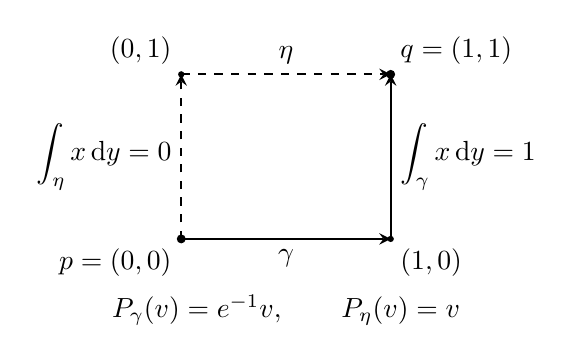
\begin{tikzpicture}[>=stealth,scale=0.95]
		\draw[thick,->] (0,0)--(2.8,0) node[midway,below] {\(\gamma\)};
		\draw[thick,->] (2.8,0)--(2.8,2.2);
		\draw[dashed,thick,->] (0,0)--(0,2.2);
		\draw[dashed,thick,->] (0,2.2)--(2.8,2.2) node[midway,above] {\(\eta\)};
		\fill (0,0) circle (1.7pt) node[below left] {\(p=(0,0)\)};
		\fill (2.8,2.2) circle (1.7pt) node[above right] {\(q=(1,1)\)};
		\fill (2.8,0) circle (1.2pt) node[below right] {\((1,0)\)};
		\fill (0,2.2) circle (1.2pt) node[above left] {\((0,1)\)};
		\node[left] at (0,1.1) {\(\displaystyle\int_\eta x\,\mathrm{d}y=0\)};
		\node[right] at (2.8,1.1) {\(\displaystyle\int_\gamma x\,\mathrm{d}y=1\)};
		\node at (1.4,-0.95) {\(P_\gamma(v)=e^{-1}v,\qquad P_\eta(v)=v\)};
	\end{tikzpicture}
	\caption{同一个联络 \(\alpha=x\,\mathrm{d}y\) 沿两条路径比较相同的两个纤维，得到不同线性同构。实线路径先水平后竖直，虚线路径的顺序相反。}
	\label{g1:fig:path-transport}
\end{figure}

\end{example}

\subsection{由平行移动恢复联络}
\label{g1:subsec:1502:03}

给定局部截面 \(S\)，式 \(S(\gamma(t))-S(\gamma(0))\) 一般没有意义，因为两个向量不在同一纤维。先用反向运输 \(P_{\gamma,0\leftarrow t}\) 把第一个向量送回起点，就能在固定向量空间中取差商。这个操作说明平行移动保存了联络的全部一阶信息。

\begin{theorem}[由运输恢复联络]\label{g1:thm:connection-from-transport}
	设 \(E\to M\) 为实有限秩光滑向量丛，\(M\) 可带边界，\(\nabla\) 为给定联络，\(P\) 是由该联络构造的平行移动。对光滑曲线 \(\gamma:I\to M\)、任意沿曲线的光滑截面 \(s\) 与固定 \(t_0\in I\)，在固定纤维 \(E_{\gamma(t_0)}\) 中有
	\begin{equation}\label{g1:eq:transported-section-derivative}
		\frac{\mathrm{d}}{\mathrm{d}t}\bigl(P_{\gamma,t_0\leftarrow t}s(t)\bigr)
		=P_{\gamma,t_0\leftarrow t}\mathrm{D}_t s.
	\end{equation}
	特别地，若 \(\gamma(0)=p\)、\(\gamma'(0)=v\)，\(S\) 是 \(p\) 附近的光滑截面，则
	\begin{equation}\label{g1:eq:connection-recovery-limit}
		(\nabla_vS)_p
		=\lim_{t\to0}\frac{P_{\gamma,0\leftarrow t}S(\gamma(t))-S(p)}{t}.
	\end{equation}
	若曲线只在零点的一侧有定义，则使用相应的单侧极限。因此同一向量丛上，若两个光滑联络沿所有分片光滑路径产生相同的平行移动，则两个联络相同。
\end{theorem}
\begin{proof}
	先在包含所考察时刻的一个标架域内计算。设从该局部初始时刻到 \(t\) 的平行移动矩阵为 \(U(t)\)，则 \(U'=-BU\)，且 \(U\) 可逆。对 \(U^{-1}U=I\) 求导，得到
	\[
		(U^{-1})'=-U^{-1}U'U^{-1}=U^{-1}B.
	\]
	若 \(s(t)=e(\gamma(t))u(t)\)，则把它运回局部初始纤维后的分量为 \(U(t)^{-1}u(t)\)，而
	\[
		\frac{\mathrm{d}}{\mathrm{d}t}(U^{-1}u)=U^{-1}(u'+Bu).
	\]
	右端恰是 \(\mathrm{D}_ts\) 反向运输后的分量。若固定的 \(t_0\) 不在这一标架域内，先运回局部初始时刻，再接上从该时刻到 \(t_0\) 的固定线性映射；固定线性映射与求导相容，故\eqref{g1:eq:transported-section-derivative}仍成立。

	现在取 \(s=S\circ\gamma\)、\(t_0=0\)，在零点求导。由 \(P_{\gamma,0\leftarrow0}=\operatorname{id}\) 及沿曲线导数与 \(\nabla_{\gamma'}S\) 的相容关系，得到\eqref{g1:eq:connection-recovery-limit}。同一局部计算也证明单侧极限的版本。

	在内部点，每个 \(v\in \mathrm{T}_pM\) 都能由坐标直线给出一条双侧小曲线的初速度，故相同的运输决定所有 \(\nabla_vS\)。在边界点取 \(x^n\ge0\)、\(x(p)=0\) 的图。若 \(v^n\ge0\)，坐标曲线 \(t\mapsto tv\)、\(t\ge0\)，留在半空间中，单侧公式决定 \(\nabla_vS\)。若 \(v^n<0\)，则 \(-v\) 是向内方向，用已经得到的值及 \(\nabla_vS=-\nabla_{-v}S\) 决定它。故两个给定联络若有相同运输，在边界点也相同。零维底流形没有非零切向方向，唯一性同样成立。
\end{proof}

边界处需要保留上述区别。一条以边界点为内部参数时刻、始终留在半空间中的双侧曲线，其法向坐标在该时刻取得局部最小值，所以法向速度必为零。不能用这种曲线代表所有切向量；向内方向由单侧曲线实现，向外方向再通过联络关于方向的线性性决定。

\ProseParagraphBreak

定理恢复的是一个已经给定的联络所产生的运输。若只向每条路径任意指定一个线性同构，即使其中部分映射满足拼接规律，也还不能直接把差商宣布为联络：差商的存在、对路径一阶信息的依赖及所需光滑性都要另外验证。本节得到的是联络与其运输之间的确定关系和唯一性。

\subsection{度量联络和长度保持}
\label{g1:subsec:1502:04}

丛度量 \(g\) 为每个纤维提供内积，存在性已由\cref{g1:thm:bundle-metric-existence}证明。但任意联络不一定在运输时保长；前面 \(x\,\mathrm{d}y\) 的例子，在标准纤维内积下就可能缩短向量。要求“沿途不变的向量保持内积”，应当对应一条关于 \(g\) 与 \(\nabla\) 的微分条件。

\begin{definition}[度量联络]\label{g1:def:metric-connection}
	设 \(E\to M\) 为实有限秩光滑向量丛，\(g\) 是光滑正定丛度量。若联络 \(\nabla\) 对所有局部向量场 \(X\) 和局部截面 \(S,T\) 满足
	\[
		X\bigl(g(S,T)\bigr)=g(\nabla_XS,T)+g(S,\nabla_XT),
	\]
	则称其为关于 \(g\) 的\term[dulianglianluo]{度量联络}[metric connection]，也称与 \(g\) 相容。这就是诱导张量联络下的 \(\nabla g=0\)。
\end{definition}

\begin{proposition}[度量相容与平行移动]\label{g1:prop:metric-parallel-transport}
	设 \(M\) 为有限维光滑流形，允许有边界，\(E\to M\) 为实有限秩光滑向量丛，带光滑正定度量 \(g\) 和联络 \(\nabla\)。以下条件等价：
	\begin{enumerate}
		\item \(\nabla g=0\)。
		\item 在每个局部标架 \(e\) 中，令 \(G=(g(e_i,e_j))\)、\(\nabla e=eA\)，则
		\begin{equation}\label{g1:eq:metric-connection-matrix}
			\mathrm{d}G=A^{\mathsf T}G+GA.
		\end{equation}
		\item 对每条光滑曲线及任意两个沿曲线的光滑截面 \(s,t\)，有
		\[
			\frac{\mathrm{d}}{\mathrm{d}\tau}g(s(\tau),t(\tau))
			=g(\mathrm{D}_\tau s,t)+g(s,\mathrm{D}_\tau t).
		\]
		\item 每条有限分片光滑路径的平行移动都是端点纤维之间的内积等距同构。
	\end{enumerate}
	因而也可以把最后一项等价地写为所有平行移动保持每个向量的长度。
\end{proposition}
\begin{proof}
	将度量相容条件应用于局部基截面 \(e_i,e_j\)。\(\nabla e_j=\sum_k e_kA^k{}_j\)，所以右边的两个矩阵分别为 \(A^{\mathsf T}G\) 和 \(GA\)，得到第二项。反过来，把任意截面写成 \(eu,ev\)，对 \(u^{\mathsf T}Gv\) 使用乘积法则，第二项就给出第一项。

	沿曲线记 \(B=A(\gamma')\)。第二项拉回曲线成为 \(G'=B^{\mathsf T}G+GB\)。于是
	\[
		\frac{\mathrm{d}}{\mathrm{d}\tau}(u^{\mathsf T}Gv)
		=(u'+Bu)^{\mathsf T}Gv+u^{\mathsf T}G(v'+Bv),
	\]
	恰为第三项。两个截面都平行时，右端为零，故内积沿每个光滑片恒定；连续性使这些常值在分段端点吻合。这证明第四项。

	反过来假设第四项。对 \(p\) 附近的局部截面 \(S,T\) 及过 \(p\) 的曲线，令
	\[
		\widehat S(\tau)=P_{\gamma,0\leftarrow\tau}S(\gamma(\tau)),\qquad
		\widehat T(\tau)=P_{\gamma,0\leftarrow\tau}T(\gamma(\tau)).
	\]
	运输保内积，故 \(g_{\gamma(\tau)}(S,T)=g_p(\widehat S(\tau),\widehat T(\tau))\)。在零点求导，再用\cref{g1:thm:connection-from-transport}，得到方向 \(v=\gamma'(0)\) 上的度量相容等式。内部点可取任意 \(v\)；边界处先取向内的单侧曲线，再利用等式两边关于 \(v\) 的线性性处理向外方向。因此第一项成立。

	最后，保内积必然保长度；反过来，实内积由
	\[
		g(v,w)=\frac12\bigl(|v+w|_g^2-|v|_g^2-|w|_g^2\bigr)
	\]
	恢复。平行移动已经线性，故保全部向量的长度也保证保内积。
\end{proof}

在正交归一标架中 \(G=I_r\)，矩阵条件简化为 \(A^{\mathsf T}+A=0\)，即每个 \(A(X)\) 为斜对称矩阵。在一般标架中却不能直接要求 \(A\) 斜对称，必须保留 \(\mathrm{d}G\) 这一项。度量可能随基点变化，而非正交标架自身的长度也会变化。

\begin{proposition}[度量联络的存在]\label{g1:prop:metric-connection-existence}
	设 \(M\) 为有限维、Hausdorff、第二可数的光滑流形，允许有边界，\(E\to M\) 为实有限秩光滑向量丛，\(g\) 为光滑正定丛度量。则 \(E\) 上存在与 \(g\) 相容的联络。给定一个度量联络后，所有其他度量联络恰为 \(\nabla+K\)，其中 \(K\in\Omega^1(M;\operatorname{End}E)\) 满足每个 \(K(X)\) 关于 \(g\) 斜伴随。
\end{proposition}
\begin{proof}
	由\cref{g1:thm:connection-existence}取任意联络 \(\nabla^0\)，再修正它不保持度量的部分。定义
	\[
		Q_X(S,T)=Xg(S,T)-g(\nabla^0_XS,T)-g(S,\nabla^0_XT).
	\]
	Leibniz 法则使这里对 \(S,T\) 的导数项在乘以函数时抵消，故 \(Q\) 对 \(X,S,T\) 都是逐点线性的；它还是光滑的，且对 \(S,T\) 对称。正定性使每个纤维的 \(g\) 非退化，因此存在唯一的 \(C_X\in\operatorname{End}(E)\)，满足
	\[
		g(C_XS,T)=\frac12Q_X(S,T).
	\]
	在局部标架中，若 \(Q_X\) 的对称矩阵为 \(Q(X)\)，这个算子为 \(C_X=\tfrac12G^{-1}Q(X)\)。矩阵逆光滑，故 \(C\) 是光滑的 \(\operatorname{End}E\) 值一形式。

	由\cref{g1:prop:connection-affine-space}，\(\nabla=\nabla^0+C\) 仍是联络。对称性给出
	\begin{align*}
		(\nabla_Xg)(S,T)&=Q_X(S,T)-g(C_XS,T)-g(S,C_XT)\\
		&=Q_X(S,T)-\tfrac12Q_X(S,T)-\tfrac12Q_X(S,T)=0.
	\end{align*}
	因此修正后的联络与度量相容。在矩阵语言中，这一修正是
	\[
		A=A^0+\frac12G^{-1}\bigl(\mathrm{d}G-(A^0)^{\mathsf T}G-GA^0\bigr).
	\]

	若 \(\widetilde\nabla=\nabla+K\)，其中 \(\nabla\) 已度量相容，则
	\[
		(\widetilde\nabla_Xg)(S,T)=-g(K(X)S,T)-g(S,K(X)T).
	\]
	因而 \(\widetilde\nabla\) 也相容，当且仅当每个 \(K(X)\) 斜伴随。这证明了最后的全部刻画。
\end{proof}

\begin{example}\label{g1:exm:rotating-metric-transport}
	在平凡二维丛中取标准内积，令
	\[
		J=\begin{pmatrix}0&-1\\1&0\end{pmatrix},\qquad A=J\,\alpha
	\]
	其中 \(\alpha\) 是任意实一形式。因为 \(J^{\mathsf T}=-J\)，这是度量联络。沿路径记 \(\theta(t)=\int_{t_0}^t \alpha(\gamma'(v))\,\mathrm{d}v\)，则
	\[
		u(t)=\exp(-\theta(t)J)u_0
		=\begin{pmatrix}\cos\theta(t)&\sin\theta(t)\\-\sin\theta(t)&\cos\theta(t)\end{pmatrix}u_0.
	\]
	矩阵求导给出 \(u'=-J\,\alpha(\gamma')u\)，因此这就是平行解。它保持长度，转角却是 \(-\theta\)，再次显示平行方程中的负号。保长不表示每条环路运输都为恒等；它只把可能的运输限制在纤维的正交变换之中。
\end{example}

% 纲要条目排为编号小节标题，并进入目录与书签；说明段仍保留于纲要注释中。
